%% -*- coding: utf-8 -*-
\documentclass[12pt,a4paper]{report}
\usepackage[left=2cm,right=2cm,
    top=2cm,bottom=2cm,bindingoffset=0cm]{geometry} 
\usepackage[utf8]{inputenc}
\usepackage[english,russian]{babel}
\usepackage{indentfirst}
\usepackage{misccorr}
\usepackage{graphicx}
\usepackage{amsmath}
\usepackage{amsfonts}
\usepackage{amssymb}
\setcounter{page}{2}
\begin{document}

\begin{titlepage}
\newpage
  \begin{center}
     
    Санкт-Петербургский Политехнический Университет Петра Великого \\
    
    Институт компьютерных наук и технологий \\
    
    Кафедра компьютерных систем и программных технологий
    \end{center}
    
    \vspace{15em}
    \begin{center}
    \textsc{Лабораторная работа №6}\\
    \vspace{5mm}
    \textsc{Цифровая модуляция}
    	
   \end{center}
\vspace{10em}

\newlength{\ML}
\settowidth{\ML}{«\underline{\hspace{0.7cm}}» \underline{\hspace{2cm}}}
\hfill\begin{minipage}{0.45\textwidth}
\vfill
  Руководитель \\
  \\
  \underline{\hspace{\ML}} Богач Н.\,В.\\
 
\end{minipage}%
\bigskip

\hfill\begin{minipage}{0.45\textwidth}
  Выполнил\\
  \\
  \underline{\hspace{\ML}} Солдатова Е.\,И.\\
  группа 33501/3
\end{minipage}%

\vspace{\fill}
\begin{center}
    
  Санкт-Петербург\\
   2018 
\end{center}
\end{titlepage}

\paragraph{1. Цель работы\\\\}
Изучение методов модуляции цифровых сигналов.

\paragraph{2. Постановка задачи\\}
\begin{enumerate}
\item Получить сигналы BPSK, PSK, OQPSK, genQAM, MSK, MFSK
модуляторов
\item Построить их сигнальные созвездия
\item Провести сравнение изученных методов модуляции цифровых
сигналов
\end{enumerate}

\paragraph{3. Теоретическая часть \\\\}

\paragraph{3. Ход работы \\\\}


Сигнальное созвездие BPSK (модуляция и демодуляция)

\begin{figure}[h!]
\center{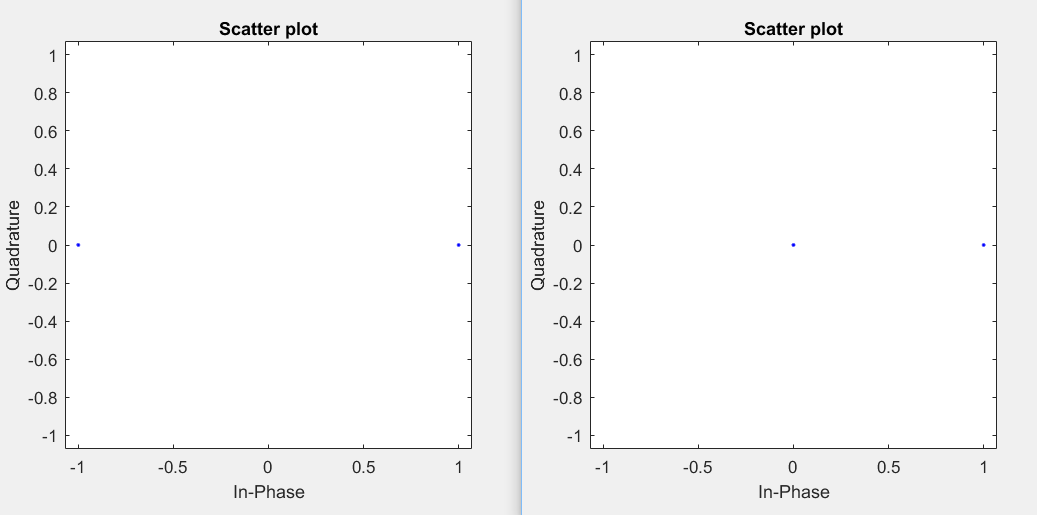
\includegraphics[width=0.7\linewidth]{bpsk}}
\end{figure}

Сигнальное созвездие PSK (модуляция и демодуляция)

\begin{figure}[h!]
\center{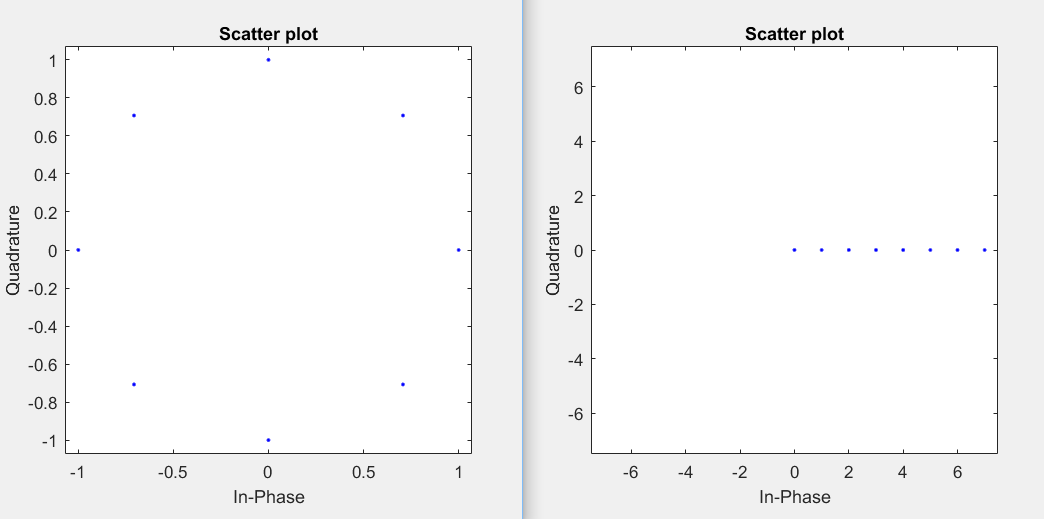
\includegraphics[width=0.7\linewidth]{psk}}
\end{figure}



\paragraph{5. Выводы \\\\}
\end{document}

